\documentclass[10pt,a4paper,titlepage,spanish]{article}
\usepackage[utf8]{inputenc}
\usepackage{amsmath}
\usepackage{amsfonts}
\usepackage{amssymb}
\usepackage{makeidx}
\usepackage{graphicx}
\usepackage{fancyheadings}  %necesitamos instalar el paquete  fancyheadings.sty
\pagestyle{fancy}
\begin{document}
\author{Luis Alberto Guanuco}
\title{Plataforma de Hardware Reconfigurable}
\date{Junio 2011}
\maketitle

\lhead{\bfseries 
\includegraphics[width=0.04\paperwidth]{logo-utn}}
\rhead{\bfseries 
\includegraphics[width=0.1\paperwidth]{logo-dpto}}
\chead{\bfseries Universida Tecnológica Nacionali\linebreak Facultad Regional Córdoba}
\lfoot{Doc.-IEPF-01-Carátula Proyecto Final \linebreak F.U.M: Mayo 2008}
\rfoot{\thepage}
\cfoot{}

\setlength{\headrulewidth}{0.4pt}

%\begin{abstract}
%El presente trabajo de tesis, enfocado en el ámbito académico, presenta una plataforma educativa abierta para el desarrollo de descripción de hardware en dispositivos PLDs (Programmable Logic Devices). El desarrollo cubre las herramientas de hardware para las Cátedras de Técnicas Digitales, lo que permite al estudiante introducirse en el diseño de arquitecturas reconfigurables. A la vez que la plataforma ayuda en el aprendizaje y puesta en práctica de los diseños descritos en VHDL(VHSIC hardware description language), permite el acercamiento a la microelectrónica, área fundamental en el desarrollo tecnológico.
%\end{abstract}

\section{Desarrollo}

El desarrollo est compuesto por una placa base que contiene todos los recursos/periféricos a ser utilizados por el dispositivo central, esto se puede ver en la Figura 1.
%

%
%\begin{figure}
%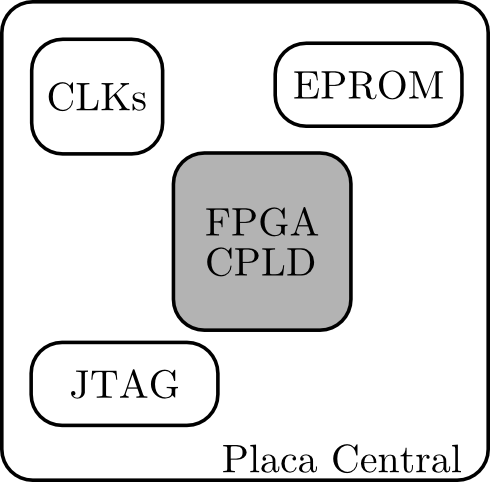
\includegraphics[width=0.2\paperwidth]{fig2}
%\caption{Placa FPGA}
%\end{figure}

El bloque central posee el dispositivo logico reconfigurable, que puede ser una FPGA o un CPLD. En la misma placa se dispone de el clock externo como tambin memoria de programación, Figura 2.
\section{Recursos}

El desarrollado del proyecto se realizar integramente en el grupo de investigacin CUDAR. El grupo est compuesto con docentes y estudiantes especializados en el área de robótica como también en la automatización de sistemas físicos empleando nuevas tecnologías. Particularmente se posee un gran conocimiento del lenguaje que permite la descripción
de hardware logrando diseñar arquitecturas reconfigurables en FPGA/CPLD.
Con el desafo de difundir ésta tecnología, CUDAR gestó la creación de la electiva \textquotedblleft{}Tcnicas Digitales IV\textquotedblright{} que se encuentra dictando ya hace cinco años con un alto acaparamiento de estudiantes avanzados de la carrera.
\section{Recursos}

El desarrollado del proyecto se realizar integramente en el grupo de investigacin CUDAR. El grupo est compuesto con docentes y estudiantes especializados en el área de robótica como también en la automatización de sistemas físicos empleando nuevas tecnologías. Particularmente se posee un gran conocimiento del lenguaje que permite la descripción
de hardware logrando diseñar arquitecturas reconfigurables en FPGA/CPLD.
Con el desafo de difundir ésta tecnología, CUDAR gestó la creación de la electiva \textquotedblleft{}Tcnicas Digitales IV\textquotedblright{} que se encuentra dictando ya hace cinco años con un alto acaparamiento de estudiantes avanzados de la carrera.
\section{Recursos}

El desarrollado del proyecto se realizar integramente en el grupo de investigacin CUDAR. El grupo est compuesto con docentes y estudiantes especializados en el área de robótica como también en la automatización de sistemas físicos empleando nuevas tecnologías. Particularmente se posee un gran conocimiento del lenguaje que permite la descripción
de hardware logrando diseñar arquitecturas reconfigurables en FPGA/CPLD.
Con el desafo de difundir ésta tecnología, CUDAR gestó la creación de la electiva \textquotedblleft{}Tcnicas Digitales IV\textquotedblright{} que se encuentra dictando ya hace cinco años con un alto acaparamiento de estudiantes avanzados de la carrera.

\setlength{\footrulewidth}{0.4pt}
\end{document}
